\documentclass[11pt,a4paper]{article}
% ==================================================================
% LogicWard — Deep Technical Report (multi-site OT drift detection)
% Compile:  pdflatex LogicWard_Technical_Report.tex   (run twice for TOC)
% ==================================================================
\usepackage[utf8]{inputenc}
\usepackage[T1]{fontenc}
\usepackage{lmodern}
\usepackage{amssymb}
\usepackage[margin=2.2cm]{geometry}
\usepackage[dvipsnames,table]{xcolor}
\usepackage{booktabs}
\usepackage{tabularx}
\usepackage{longtable}
\usepackage{array}
\usepackage{listings}
\usepackage{titlesec}
\usepackage{enumitem}
\usepackage{fancyhdr}
\setlength{\headheight}{24pt}
\addtolength{\topmargin}{-10pt}
\usepackage{parskip}
\usepackage[most]{tcolorbox}
\usepackage{tikz}
\usetikzlibrary{arrows.meta,positioning,shapes.geometric,backgrounds,fit,calc}
\usepackage{underscore}
\usepackage[hidelinks]{hyperref}

% ---------------- palette ----------------
\definecolor{navy}{HTML}{14304F}
\definecolor{navy2}{HTML}{1D4370}
\definecolor{accent}{HTML}{3987E5}
\definecolor{ink}{HTML}{1F2937}
\definecolor{muted}{HTML}{5B6B80}
\definecolor{good}{HTML}{0E7A0E}
\definecolor{warn}{HTML}{A16207}
\definecolor{serious}{HTML}{C05621}
\definecolor{critical}{HTML}{C02626}
\definecolor{page}{HTML}{EEF0F4}
\definecolor{hair}{HTML}{DBE0E8}
\definecolor{codebg}{HTML}{F6F8FB}
\definecolor{chem}{HTML}{A16207}

\hypersetup{colorlinks=true,linkcolor=navy2,urlcolor=accent}

\titleformat{\section}{\Large\bfseries\color{navy}}{\thesection}{0.6em}{}
\titleformat{\subsection}{\large\bfseries\color{navy2}}{\thesubsection}{0.6em}{}
\titleformat{\subsubsection}{\normalsize\bfseries\color{ink}}{\thesubsubsection}{0.6em}{}
\titlespacing*{\section}{0pt}{1.4em}{0.6em}

\pagestyle{fancy}
\fancyhf{}
\renewcommand{\headrulewidth}{0.4pt}
\renewcommand{\headrule}{\hbox to\headwidth{\color{hair}\leaders\hrule height \headrulewidth\hfill}}
\fancyhead[L]{\small\color{muted}\textbf{LogicWard}\,\textbullet\, Multi-Site OT Drift Detection}
\fancyhead[R]{\small\color{muted}Technical Report}
\fancyfoot[C]{\small\color{muted}\thepage}

\lstdefinestyle{lw}{basicstyle=\ttfamily\small\color{ink},backgroundcolor=\color{codebg},
  frame=single,framesep=6pt,rulecolor=\color{hair},breaklines=true,columns=fullflexible,
  keepspaces=true,showstringspaces=false,xleftmargin=4pt,xrightmargin=4pt,aboveskip=8pt,belowskip=8pt}
\lstset{style=lw}

\newtcolorbox{keybox}[1][]{colback=accent!6,colframe=accent,boxrule=0.8pt,left=8pt,right=8pt,top=6pt,bottom=6pt,arc=2pt,#1}
\newtcolorbox{warnbox}[1][]{colback=critical!5,colframe=critical,boxrule=0.8pt,left=8pt,right=8pt,top=6pt,bottom=6pt,arc=2pt,#1}
\newcommand{\code}[1]{\texttt{\small #1}}
\newcolumntype{L}{>{\raggedright\arraybackslash}X}
% ER-entity helpers (used inside TikZ nodes)
\newcommand{\enthead}[1]{\colorbox{navy}{\color{white}\bfseries\sffamily #1}}
\newcommand{\entrow}[1]{{\footnotesize\ttfamily\color{ink}#1}}

% ---------------- TikZ shared styles ----------------
\tikzset{
  box/.style   = {rectangle, rounded corners=3pt, draw=navy!70, fill=navy!5, line width=0.7pt,
                  text=ink, align=center, font=\small\sffamily, inner sep=6pt, minimum height=9mm},
  accbox/.style= {box, draw=accent, fill=accent!8},
  redbox/.style= {box, draw=critical, fill=critical!7},
  chembox/.style={box, draw=chem, fill=chem!8},
  goodbox/.style={box, draw=good, fill=good!8},
  ent/.style   = {rectangle, draw=navy2, fill=navy!6, line width=0.7pt, align=center,
                  font=\small\sffamily, inner sep=0pt, minimum width=34mm},
  fl/.style    = {-{Latex[length=2.4mm]}, line width=0.8pt, draw=navy2},
  flr/.style   = {-{Latex[length=2.4mm]}, line width=0.8pt, draw=critical},
  lbl/.style   = {font=\scriptsize\sffamily, text=muted, fill=white, inner sep=1.5pt},
}

% ==================================================================
\begin{document}

% ---------------- title page ----------------
\begin{titlepage}
\thispagestyle{empty}
\vspace*{1.1cm}
{\color{navy}\rule{\textwidth}{2.5pt}}\\[0.5cm]
{\Huge\bfseries\color{navy} LogicWard}\\[0.30cm]
{\LARGE\color{navy2} Live OT Drift-Detection \& Incident-Response Platform}\\[0.20cm]
{\large\color{muted} A unified, multi-site fabric that detects unauthorized PLC logic and\\
process drift \emph{before} it becomes operational or safety risk.}\\[1.0cm]

\begin{tcolorbox}[colback=accent!6,colframe=accent,boxrule=1pt,arc=3pt,left=12pt,right=12pt,top=10pt,bottom=10pt]
\color{ink}\small
\textbf{Two monitored plants, one detection fabric:}\\[3pt]
\textbf{Site A — Thermal Power Plant} (Raspberry Pi PLC, Rockwell L5X ladder, animated SCADA mimic)\\
\textbf{Site B — GRFICS Chemical Reactor} (OpenPLC Structured Text, live Unity 3D digital twin)\\[5pt]
Every attack traverses the full lifecycle: \emph{Execution $\rightarrow$ Register change $\rightarrow$ 3D/gauge update $\rightarrow$
Drift detection $\rightarrow$ Alert $\rightarrow$ Evidence $\rightarrow$ MITRE ATT\&CK for ICS $\rightarrow$ Timeline $\rightarrow$ Response $\rightarrow$ Rollback.}
\end{tcolorbox}

\vfill
{\color{muted}\small
\textbf{Technical Report} \textbullet\ Architecture, Data Model, Detection, Attacks, RBAC \& Deployment\\
Prepared for the Adani OT Cybersecurity demonstration \textbullet\ \today}\\[0.3cm]
{\color{navy}\rule{\textwidth}{2.5pt}}
\end{titlepage}

\tableofcontents
\newpage

% ==================================================================
\section{Executive Summary}
Operational-Technology (OT) attacks do not announce themselves. A single unauthorized
change to a Programmable Logic Controller (PLC) --- a lowered trip setpoint, an inverted
safety comparator, a hijacked output coil --- can sit invisibly in a running plant until it
causes a trip, a spill, or a catastrophe. \textbf{LogicWard} is a live drift-detection
appliance that watches the running control logic and the live process state, and raises
\emph{severity-ranked, MITRE-mapped, evidence-backed} alerts the instant either drifts from a
cryptographically signed, approved baseline.

The platform is deliberately \textbf{multi-site and multi-vendor}. It simultaneously monitors a
\emph{thermal power plant} on real Raspberry Pi hardware (Rockwell L5X ladder logic) and a
\emph{chemical reactor} rendered as a live Unity 3D digital twin (OpenPLC Structured Text),
proving that the detection fabric is \emph{process-agnostic}: the same event bus, severity model,
MITRE mapping and evidence log serve two entirely different plants under one SOC console.

\begin{keybox}
\textbf{The prime architectural invariant.} The PLC ``program'' is \textbf{data to baseline,
diff and mutate --- it is never executed.} LogicWard does not interpret ladder logic; the live
Modbus registers provide the physical reality underneath. This is what keeps the appliance
safe, fast and false-positive-free.
\end{keybox}

\subsection{Headline capabilities}
\begin{itemize}[leftmargin=1.3em,itemsep=2pt]
  \item \textbf{Structural + register drift detection} against an HMAC-SHA256 signed baseline,
        naming six PLC mutations plus raw register/coil tampering.
  \item \textbf{Unified event fabric} --- one \code{Event} contract, three detection planes
        (cyber / physical / resource), enriched on emit with severity, identity and MITRE.
  \item \textbf{Two live plants} under one dashboard with a site selector, a shared alert
        timeline, and per-site forensic PDF export.
  \item \textbf{Twelve real attacks} (7 thermal, 5 chemical) fired from a red-team console over
        genuine unauthenticated Modbus / program-download channels.
  \item \textbf{Production-grade SOC UI} --- risk score, attack timeline, system health,
        rollback status, live trend sparklines.
  \item \textbf{Capability-based RBAC} across six OT/ICS roles, enforced server- and client-side.
  \item \textbf{154 automated integration checks} across nine suites.
\end{itemize}

% ==================================================================
\section{Problem Statement \& Threat Model}
\subsection{Why OT drift is hard}
IT security assumes patchable, observable, restartable assets. OT inverts every assumption:
PLCs run unauthenticated legacy protocols (Modbus has no authentication), cannot be patched
mid-process, and a ``reboot'' may mean a plant trip. The adversary's goal is rarely data theft;
it is \emph{physical consequence} --- defeat a safety interlock, then let physics do the damage.

\subsection{Adversary capabilities modelled}
\begin{itemize}[leftmargin=1.3em,itemsep=2pt]
  \item \textbf{Unauthenticated Modbus writes} (FC05/FC06/FC10) --- move setpoints, force coils.
  \item \textbf{Engineering-workstation compromise} --- download a mutated PLC program.
  \item \textbf{Network foothold} --- rogue master / device on the OT segment; denial of service.
  \item \textbf{Physical access} --- cabinet tamper, cable pull (physical plane).
\end{itemize}

\subsection{Detection philosophy}
LogicWard assumes the attacker is \emph{already inside} and can write to the PLC. It does not
try to keep them out; it makes any deviation from the approved state \emph{immediately visible,
attributable and reversible}. Detection is a structural \emph{diff}, not anomaly-guessing ---
which is why a harmless program re-export (new timestamps, same logic) hashes identically and
raises nothing, while a real logic change is caught on the first scan.

% ==================================================================
\section{System Architecture}
LogicWard is a Python package (\code{logicward/}) built on Flask and a raw-socket Modbus stack.
Figure~\ref{fig:arch} shows the end-to-end fabric: red-team attack channels on the left, the two
monitored sites in the middle, and the shared detection/evidence/presentation plane on the right.

\begin{figure}[h]
\centering
\begin{tikzpicture}[node distance=6mm and 12mm]
% attackers
\node[redbox] (atk) {Attacker Console\\\scriptsize (Red Team, :9090)};
% sites
\node[box, right=22mm of atk, yshift=12mm] (pi) {\textbf{Site A — Thermal (Pi)}\\\scriptsize Modbus PLC :5020\\\scriptsize L5X program :8081};
\node[chembox, right=22mm of atk, yshift=-12mm] (chem) {\textbf{Site B — Chemical (3D)}\\\scriptsize Modbus PLC :5021\\\scriptsize Unity feed / \texttt{/data}};
% engine
\node[accbox, right=16mm of pi, yshift=-12mm] (eng) {Drift Engine\\\scriptsize structural + register};
\node[accbox, below=10mm of eng] (bus) {\textbf{Event Bus}\\\scriptsize severity + MITRE + identity};
% sinks
\node[box, right=14mm of eng] (dash) {SOC Dashboard\\\scriptsize (:8080, RBAC)};
\node[goodbox, right=14mm of bus] (ev) {Evidence Log\\\scriptsize JSONL + signed PDF};
% edges
\draw[flr] (atk) -- node[lbl,above,sloped]{Modbus write} (pi);
\draw[flr] (atk) -- node[lbl,below,sloped]{Modbus write} (chem);
\draw[fl] (pi) -- node[lbl,above,sloped]{poll} (eng);
\draw[fl] (chem) -- node[lbl,below,sloped]{poll} (eng);
\draw[fl] (eng) -- (bus);
\draw[fl] (bus) -- (dash.west|-bus);
\draw[fl] (eng) -- (dash);
\draw[fl] (bus) -- (ev);
\draw[fl,dashed] (dash) to[bend left=18] node[lbl,right]{restore / quarantine} (bus);
\end{tikzpicture}
\caption{End-to-end architecture. Attacks are real unauthenticated writes; both plants are polled
by one transport-agnostic drift engine that feeds a single enriched event bus, which fans out to
the evidence log and the role-gated SOC dashboard.}
\label{fig:arch}
\end{figure}

\subsection{The event bus is the spine}
Every detector --- cyber, physical, resource, and the response engine --- emits the \emph{same}
\code{Event} object. On \code{emit()} the bus validates, is idempotent by \code{event_id},
enriches (computes severity, attaches MITRE, identity, sequence), and fans out to three sinks:
the append-only JSONL evidence log, the dashboard poll buffer, and live subscribers.

\begin{lstlisting}
Event = {
  event_id, type,            # e.g. "cyber.setpoint_drift" | "physical.rogue_device"
  timestamp, source, severity,
  details { ... , site },    # site attributes the event to a plant
  identity { who, mac, channel },
  mitre { tactic, technique_id, technique_name, verified },
  seq, received_at
}
\end{lstlisting}

\subsection{The site abstraction (process-agnostic)}
A single seam --- \code{engine/sources.py} --- makes the engine transport- and process-agnostic:
it only needs \code{program\_source() -> bytes} and \code{register\_source() -> \{holding, coils\}}.
\code{EmbeddedPlant} runs an in-process PLC (one-machine dev/demo); \code{RemotePlant} reads a real
Pi over Modbus + HTTP. Site B (\code{sites/grfics/}) plugs into the same seam as a second site.

% ==================================================================
\section{Multi-Site Model}
\begin{table}[h]\small
\centering
\renewcommand{\arraystretch}{1.25}
\begin{tabularx}{\textwidth}{@{}l L L@{}}
\toprule
 & \textbf{Site A — Thermal Power Plant} & \textbf{Site B — GRFICS Chemical Reactor}\\
\midrule
Hardware & Raspberry Pi (real) & Laptop (simulated) \\
Vendor / program & Rockwell \textbf{L5X} ladder & OpenPLC \textbf{Structured Text} \\
Detection surface & structural (program) + register & register plane \\
Visualization & animated SVG SCADA mimic & live \textbf{Unity 3D} digital twin \\
Modbus & TCP :5020 (unauthenticated) & TCP :5021 (unauthenticated) \\
Site id & \code{thermal-pi} & \code{grfics-chem} \\
\bottomrule
\end{tabularx}
\caption{The two monitored sites. Both feed one bus; events are attributed via \code{details.site}.}
\end{table}

\begin{keybox}
\textbf{Why this matters for the pitch.} The claim is not ``I detect drift on my simulator.'' It
is ``I detect drift across \emph{vendors, programming languages and physical processes} on one
fabric.'' Adding a water plant or a substation is a new \emph{site profile}, not a rewrite.
\end{keybox}

% ==================================================================
\section{Attack Lifecycle \& Data Flow}
Every attack --- on either site --- traverses the same ten-stage lifecycle (Figure~\ref{fig:flow}).
This is the backbone of the demonstration: an observer can point to each stage on screen.

\begin{figure}[h]
\centering
\begin{tikzpicture}[node distance=4.5mm and 7mm, every node/.style={font=\scriptsize\sffamily}]
\node[redbox]  (a) {1. Attack\\Execution};
\node[chembox, right=of a] (b) {2. PLC /\\Register change};
\node[box, right=of b]     (c) {3. 3D + Gauge\\update};
\node[accbox, right=of c]  (d) {4. Drift\\Detection};
\node[accbox, right=of d]  (e) {5. Event Bus\\severity+MITRE};
\node[goodbox, below=9mm of e] (f) {6. Evidence\\collected};
\node[box, left=of f]      (g) {7. Timeline\\update};
\node[box, left=of g]      (h) {8. Alert\\raised};
\node[box, left=of h]      (i) {9. Operator\\response};
\node[goodbox, left=of i]  (j) {10. Rollback /\\recovery};
\draw[flr](a)--(b); \draw[fl](b)--(c); \draw[fl](c)--(d); \draw[fl](d)--(e);
\draw[fl](e)--(f); \draw[fl](f)--(g); \draw[fl](g)--(h); \draw[fl](h)--(i); \draw[fl](i)--(j);
\draw[fl,dashed](j) to[bend left=22] node[lbl,above]{baseline restored} (b);
\end{tikzpicture}
\caption{The ten-stage attack lifecycle every scenario follows. Stages 4--7 are the automated
LogicWard core; stages 9--10 are the role-gated response (acknowledge, quarantine, safe-state,
restore baseline).}
\label{fig:flow}
\end{figure}

% ==================================================================
\section{Detection Engine}
Detection runs in a one-second loop with two surfaces.

\subsection{Structural (program) detection}
The live L5X is parsed and \emph{canonicalized} (\code{engine/l5x.py}): volatile attributes
(export/edit dates, revisions, CRC, comments) are stripped, neutral-text ladder such as
\code{XIC(..)[LES(..)]OTE(..);} is parsed into instruction/operand structs, and a
\code{structural\_hash} is produced. A rung-by-rung diff against the signed baseline names six
mutations:

\begin{table}[h]\small\centering
\renewcommand{\arraystretch}{1.2}
\begin{tabularx}{\textwidth}{@{}l L l l@{}}
\toprule
\textbf{Mutation} & \textbf{Meaning} & \textbf{Severity} & \textbf{MITRE ICS}\\
\midrule
\code{condition\_stripping} & safety input removed from a rung & critical & T0889 \\
\code{logic\_inversion}     & comparator/contact flipped (LES$\leftrightarrow$GRT) & critical & T0889 \\
\code{coil\_hijack}         & output coil repointed to another actuator & critical & T0889 \\
\code{rung\_injection}      & unauthorized new rung added & high & T0843 \\
\code{setpoint\_drift}      & threshold / setpoint tag value changed & high & T0836 \\
\code{register\_change}     & raw holding-register / coil write over Modbus & low--med & T0855 \\
\bottomrule
\end{tabularx}
\caption{The six named mutations, their severity band and verified MITRE ATT\&CK for ICS technique.}
\end{table}

\subsection{Register (process) detection}
Live Modbus holding registers and control coils are diffed against the baseline snapshot. Input
registers (sensor values) are \emph{intentionally not} diffed --- they carry live process noise;
only operator-controllable holdings and coils are integrity-checked, which is why the plant sits
silent at rest and only speaks when tampered.

\subsection{Signed baseline \& tamper detection}
The approved configuration (program + structural hash + setpoints + register snapshot) is captured
into a manifest and signed with \textbf{HMAC-SHA256} (\code{engine/baseline.py}). Editing the locked
manifest breaks the signature; a \code{watchdog} file-integrity monitor watches both the live
program file and the signed baseline and re-verifies on change. This is integrity, not access
control --- and it is honestly framed as such.

% ==================================================================
\section{Attack Catalogue}
Twelve real attacks fire over genuine channels. Thermal program mutations use the unauthenticated
program-download endpoint; register/coil attacks use raw Modbus.

\subsection{Site A --- Thermal (7)}
\begin{table}[h]\small\centering
\renewcommand{\arraystretch}{1.15}
\begin{tabularx}{\textwidth}{@{}l l L l@{}}
\toprule
\textbf{Attack} & \textbf{Channel} & \textbf{Effect} & \textbf{MITRE}\\
\midrule
Setpoint Drift & Modbus FC06 & Drum-level trip setpoint 220$\to$40\,mm (blinds protection) & T0836\\
Logic Inversion & Program & drum-level comparator LES$\to$GRT (trips backwards) & T0889\\
Condition Stripping & Program & remove \code{Plant\_Running} interlock from fuel trip & T0889\\
Coil Hijack & Program & repoint \code{Feedwater\_Trip}$\to$\code{Cooling\_Pump\_Stop} & T0889\\
Rung Injection & Program & inject backdoor rung unlatching turbine overspeed trip & T0843\\
Force Coil & Modbus FC05 & force \code{Fuel\_Valve\_Open} off (flame-loss trip) & T0855\\
DDoS Flood & Modbus FC03 & multi-threaded read flood, CPU spike & T0814\\
\bottomrule
\end{tabularx}
\end{table}

\subsection{Site B --- Chemical (5, demo-ordered, blast last)}
Each chemical attack drives a \emph{distinct} live signature on the SOC gauges (and, where the
compiled Unity binary supports it, on the 3D scene). They are ordered for a live pitch that
escalates to a catastrophic finale.

\begin{table}[h]\small\centering
\renewcommand{\arraystretch}{1.15}
\begin{tabularx}{\textwidth}{@{}c l L l@{}}
\toprule
\textbf{\#} & \textbf{Attack} & \textbf{Distinct signature} & \textbf{MITRE}\\
\midrule
1 & Quality Sabotage & feed ratio skewed; composition/colour shifts, no alarm (stealth) & T0855\\
2 & Feed Pump Trip & pump 1 off; reactor starved, liquid level \emph{drains} & T0855\\
3 & Tank Overfill & product shut, feeds high; level \emph{rises} to overflow + trip & T0855\\
4 & E-Stop Injection & ESD coil forced; plant halts, all valves safe-state & T0855\\
5 & \textbf{Pressure Redline (BLAST)} & \emph{all} trips defeated + feeds open + purge shut; pressure to the ceiling --- the reactor \textbf{blasts} & T0836\\
\bottomrule
\end{tabularx}
\end{table}

\begin{warnbox}
\textbf{Honest 3D limitation.} The GRFICS Unity scene is a \emph{pre-compiled WebGL binary}; its
process animations (liquid level, colour) are driven only where the binary already maps the JSON
keys. The pressure explosion animates; level/colour depend on the binary and are fully solved by a
Unity recompile. \emph{All} per-attack distinctiveness is guaranteed on the live SOC gauges,
detection feed and timeline --- where the telemetry is actually read during a pitch.
\end{warnbox}

% ==================================================================
\section{Data Model (Entity--Relationship)}
LogicWard's runtime state is a small, clean model (Figure~\ref{fig:er}). \code{Event} is the
central entity; \code{Site} attributes it to a plant; \code{Baseline} is the signed reference the
drift engine diffs against; \code{User}$\to$\code{Role}$\to$\code{Capability} governs access.

\begin{figure}[h]
\centering
\begin{tikzpicture}[node distance=10mm and 20mm]
% EVENT entity
\node[ent] (event) {
  \begin{tabular}{@{}c@{}}
  \enthead{\makebox[34mm]{EVENT}}\\[1pt]
  \entrow{event_id (PK)}\\ \entrow{type}\\ \entrow{severity}\\ \entrow{timestamp}\\
  \entrow{details\{\}}\\ \entrow{mitre\{\}}\\ \entrow{identity\{\}}\\ \entrow{seq}
  \end{tabular}};
% SITE
\node[ent, above right=2mm and 26mm of event] (site) {
  \begin{tabular}{@{}c@{}}
  \enthead{\makebox[34mm]{SITE}}\\[1pt]
  \entrow{site_id (PK)}\\ \entrow{name}\\ \entrow{vendor}\\ \entrow{protocol}\\
  \entrow{program_type}\\ \entrow{viz_type}
  \end{tabular}};
% BASELINE
\node[ent, below right=2mm and 26mm of event] (base) {
  \begin{tabular}{@{}c@{}}
  \enthead{\makebox[34mm]{BASELINE}}\\[1pt]
  \entrow{structural_hash (PK)}\\ \entrow{l5x program}\\ \entrow{setpoints\{\}}\\
  \entrow{registers\{\}}\\ \entrow{hmac_signature}
  \end{tabular}};
% USER / ROLE / CAP (right column)
\node[ent, right=40mm of site] (user) {
  \begin{tabular}{@{}c@{}}
  \enthead{\makebox[30mm]{USER}}\\[1pt]
  \entrow{username (PK)}\\ \entrow{name}\\ \entrow{role_id (FK)}
  \end{tabular}};
\node[ent, below=12mm of user] (role) {
  \begin{tabular}{@{}c@{}}
  \enthead{\makebox[30mm]{ROLE}}\\[1pt]
  \entrow{role_id (PK)}\\ \entrow{label}
  \end{tabular}};
\node[ent, below=12mm of role] (cap) {
  \begin{tabular}{@{}c@{}}
  \enthead{\makebox[30mm]{CAPABILITY}}\\[1pt]
  \entrow{cap (PK)}\\ \entrow{gated_route}
  \end{tabular}};
% relationships
\draw[fl] (event) -- node[lbl,above,sloped]{occurs at (N:1)} (site);
\draw[fl] (event) -- node[lbl,below,sloped]{diffed vs (N:1)} (base);
\draw[fl] (user)  -- node[lbl,right]{has (N:1)} (role);
\draw[fl] (role)  -- node[lbl,right]{grants (M:N)} (cap);
\end{tikzpicture}
\caption{Runtime data model. Events are attributed to a Site and diffed against a signed Baseline;
access is a User$\to$Role$\to$Capability chain (capability, not rank).}
\label{fig:er}
\end{figure}

% ==================================================================
\section{Role-Based Access Control}
Access is \textbf{capability-based}, not a linear rank, because the six OT/ICS roles have different
\emph{scopes} --- a Network Engineer may quarantine a rogue device but must not touch the PLC
program; a Control Engineer is the reverse. Every action is gated server-side (HTTP 403) and
client-side (the control is removed from the DOM).

\begin{table}[h]\footnotesize\centering
\renewcommand{\arraystretch}{1.2}
\setlength{\tabcolsep}{4pt}
\begin{tabular}{@{}l l c c c c c c@{}}
\toprule
\textbf{Role (login)} & \textbf{Scope} & ack & ack all & baseline & net.\ resp. & safe-state & evidence\\
\midrule
Operator \code{(operator)}        & control room       & \checkmark & \checkmark &            &            &            & \\
Control Engineer \code{(engineer)}& PLC program        & \checkmark & \checkmark & \checkmark &            & \checkmark & \\
Network Engineer \code{(netsec)}  & infrastructure     & \checkmark & \checkmark &            & \checkmark &            & \\
SOC Analyst \code{(soc)}          & oversight          & \checkmark & \checkmark &            & \checkmark & \checkmark & \checkmark\\
Vendor / OEM \code{(vendor)}      & scoped, read-only  &            &            &            &            &            & \\
CISO \code{(ciso)}                & full authority     & \checkmark & \checkmark & \checkmark & \checkmark & \checkmark & \checkmark\\
\bottomrule
\end{tabular}
\caption{Capability matrix for the six roles (verified end-to-end). Vendor is deliberately
read-only and heavily monitored; CISO holds full cross-role authority.}
\end{table}

% ==================================================================
\section{MITRE ATT\&CK for ICS Mapping}
Mapping is a rule-based, explainable table (\code{engine/mitre_map.py}), verified against the live
ICS matrix. Where no technique honestly fits (physical enclosure tamper, baseline-integrity
tamper) it is marked \code{N/A} rather than assigned a fabricated ID.

\begin{table}[h]\small\centering
\renewcommand{\arraystretch}{1.2}
\begin{tabularx}{\textwidth}{@{}l l l L@{}}
\toprule
\textbf{Technique} & \textbf{ID} & \textbf{Tactic} & \textbf{LogicWard event types}\\
\midrule
Modify Parameter & T0836 & Impair Process Control & \code{cyber.setpoint\_drift}\\
Unauthorized Command Message & T0855 & Impair Process Control & \code{cyber.register\_change}\\
Modify Program & T0889 & Persistence & inversion, stripping, coil hijack\\
Program Download & T0843 & Lateral Movement & \code{cyber.rung\_injection}\\
Rogue Master & T0848 & Initial Access & \code{physical.rogue\_device}\\
Denial of Service & T0814 & Inhibit Response Function & DDoS, link down, CPU spike\\
\bottomrule
\end{tabularx}
\caption{Verified ATT\&CK for ICS techniques and the events that map to them.}
\end{table}

% ==================================================================
\section{SOC Dashboard \& Analytics}
The Flask dashboard (\code{:8080}) polls \code{/api/events?since=} and \code{/api/plant} (\raise.17ex\hbox{$\scriptstyle\sim$}1\,s;
deliberately no WebSockets, for demo robustness) and presents a production-grade console:
\begin{itemize}[leftmargin=1.3em,itemsep=2pt]
  \item \textbf{Risk Score} --- explainable 0--100 platform score (severity-weighted active alerts
        + baseline/program posture) with a LOW$\to$CRITICAL band.
  \item \textbf{Attack Timeline} --- severity-coloured temporal strip of events, site-filtered.
  \item \textbf{System Health} --- per-site online status + event rollup (NOMINAL/WARNING/CRITICAL).
  \item \textbf{Baseline \& Rollback status} --- integrity, program drift count, restore availability.
  \item \textbf{Live trend sparklines} --- rolling 60-sample history for the key thermal values.
  \item \textbf{Animated SCADA mimic} (thermal) --- each event maps to a diagram node and redlines it
        with a pinned MITRE badge; click to acknowledge.
  \item \textbf{Live 3D digital twin} (chemical) --- the Unity reactor beside live gauges.
  \item \textbf{Site selector} --- Thermal / Chemical / All, driving one common alert timeline.
\end{itemize}

% ==================================================================
\section{Deployment Topology}
The demonstration runs on a laptop plus one Raspberry Pi over a LAN (Figure~\ref{fig:deploy}).
The laptop hosts the SOC dashboard, the attacker console and the (local) chemical plant; the Pi
runs the real thermal PLC, program endpoints and a sensor agent that POSTs physical/resource
events back to the laptop's ingest endpoint.

\begin{figure}[h]
\centering
\begin{tikzpicture}[node distance=8mm and 18mm]
\begin{scope}[on background layer]
\node[draw=hair, fill=page, rounded corners, inner sep=8mm, label={[muted,font=\small\sffamily]above:Laptop}] (lap) {};
\end{scope}
\node[box] (soc) {SOC Dashboard\\\scriptsize :8080 + /api/ingest};
\node[redbox, below=of soc] (atk) {Attacker Console\\\scriptsize :9090};
\node[chembox, right=14mm of soc] (chp) {Chemical PLC + 3D\\\scriptsize :5021 + /viz};
\node[fit=(soc)(atk)(chp), draw=hair, fill=page, rounded corners, inner sep=6mm] (lapbox) {};
\node[muted,font=\small\sffamily] at ([yshift=4mm]lapbox.north) {Demo Laptop};
% Pi
\node[box, right=42mm of chp] (pi) {\textbf{Raspberry Pi}\\\scriptsize Thermal PLC :5020\\\scriptsize program :8081\\\scriptsize sensor agent};
% edges
\draw[fl] (pi.west) -- node[lbl,above]{Modbus + program (poll)} (chp.east|-pi.west);
\draw[fl,dashed] (pi) to[bend right=20] node[lbl,below]{agent POST events} (soc.east);
\draw[flr] (atk.east) -- node[lbl,below,sloped]{attack} (chp.south);
\draw[flr] (atk) to[bend right=30] node[lbl,below]{attack Pi} (pi.south);
\end{tikzpicture}
\caption{Two-machine deployment. Set \code{LOGICWARD\_MULTISITE=0} on the Pi (thermal only);
the laptop runs the unified dashboard, the red-team console and the chemical digital twin.}
\label{fig:deploy}
\end{figure}

% ==================================================================
\section{Verification \& Results}
LogicWard ships with \textbf{nine standalone integration suites --- 154 checks} --- that spin up
real servers on ephemeral ports and exercise real HTTP/Modbus paths (integration, not unit tests).

\begin{table}[h]\small\centering
\renewcommand{\arraystretch}{1.15}
\begin{tabular}{@{}l r l@{}}
\toprule
\textbf{Suite} & \textbf{Checks} & \textbf{Covers}\\
\midrule
\code{smoke\_bus}       & 15 & event contract, severity, MITRE, evidence, idempotency\\
\code{smoke\_l5x}       & 16 & L5X parse, canonicalize, structural hash\\
\code{smoke\_plant}     & 14 & thermal Modbus server + setpoint-driven trips\\
\code{smoke\_drift}     & 18 & six mutations + register diff, no false positives\\
\code{smoke\_agent}     & 10 & physical/resource sensors + forwarder\\
\code{smoke\_dashboard} & 15 & routes, RBAC (403 gating), response actions\\
\code{smoke\_attacker}  & 10 & attack framework + mutators\\
\code{smoke\_grfics}    & 36 & 5 distinct chemical attacks, each own signature\\
\code{smoke\_multisite} & 20 & unified feed, per-site evidence, attacker both sites\\
\midrule
\textbf{Total} & \textbf{154} & \\
\bottomrule
\end{tabular}
\caption{The full verification matrix. Every attack's detection, severity, MITRE and site-tagging
is asserted; the chemical suite proves all five attacks produce distinct signatures.}
\end{table}

% ==================================================================
\section{Roadmap}
\begin{itemize}[leftmargin=1.3em,itemsep=2pt]
  \item \textbf{Structured-Text program-drift} for the chemical PLC (a second \code{ProgramParser}
        behind the same canonical rung model --- the six mutations apply unchanged).
  \item \textbf{Unity recompile} to hook liquid level / composition colour / e-stop strobes to the
        already-published JSON keys, unlocking full 3D per-attack animation.
  \item \textbf{New site profiles} --- water treatment, electrical substation --- as drop-in plugins.
  \item \textbf{ML-assisted risk scoring} layered above the explainable rule-based core.
\end{itemize}

\vfill
\begin{center}\small\color{muted}
LogicWard --- one detection fabric, many plants. \textbullet\ Research-grade, demonstration-ready.
\end{center}

\end{document}
